
%(BEGIN_QUESTION)
% Copyright 2010, Tony R. Kuphaldt, released under the Creative Commons Attribution License (v 1.0)
% This means you may do almost anything with this work of mine, so long as you give me proper credit

Calculate the amount of voltage ``seen'' by the voltmeter given the following measurement and reference junction temperatures:

$$\includegraphics[width=15.5cm]{i02947x01.eps}$$

\begin{itemize}
\item{} $T_{1}$ = 589 $^{o}$F ; $T_{2}$ = 63 $^{o}$F ; $T_3$ = 70 $^{o}$F ; $V_{meter}$ = \underbar{\hskip 50pt} mV
\vskip 10pt
\item{} $T_{1}$ = 821 $^{o}$F ; $T_{2}$ = 69 $^{o}$F ; $T_3$ = 73 $^{o}$F ; $V_{meter}$ = \underbar{\hskip 50pt} mV
\vskip 10pt
\item{} $T_{1}$ = 1524 $^{o}$F ; $T_{2}$ = 91 $^{o}$F ; $T_3$ = 105 $^{o}$F ; $V_{meter}$ = \underbar{\hskip 50pt} mV
\vskip 10pt
\item{} $T_{1}$ = 1922 $^{o}$F ; $T_{2}$ = 102 $^{o}$F ; $T_3$ = 135 $^{o}$F ; $V_{meter}$ = \underbar{\hskip 50pt} mV
\end{itemize}

\underbar{file i02947}
%(END_QUESTION)





%(BEGIN_ANSWER)

All answers based on ITS-90 thermocouple table values:

\begin{itemize}
\item{} $T_{1}$ = 589 $^{o}$F ; $T_{2}$ = 63 $^{o}$F ; $T_3$ = 70 $^{o}$F ; $V_{meter}$ = {\bf 0.463} mV
\vskip 10pt
\item{} $T_{1}$ = 821 $^{o}$F ; $T_{2}$ = 69 $^{o}$F ; $T_3$ = 73 $^{o}$F ; $V_{meter}$ = {\bf 0.953} mV
\vskip 10pt
\item{} $T_{1}$ = 1524 $^{o}$F ; $T_{2}$ = 91 $^{o}$F ; $T_3$ = 105 $^{o}$F ; $V_{meter}$ = {\bf 3.378} mV
\vskip 10pt
\item{} $T_{1}$ = 1922 $^{o}$F ; $T_{2}$ = 102 $^{o}$F ; $T_3$ = 135 $^{o}$F ; $V_{meter}$ = {\bf 5.294} mV
\end{itemize}

Note: all temperatures at $T_2$ are irrelevant because this is a junction between similar metals (type B wires connecting to corresponding type B wires).  The reference (cold) junction is where the type B wires connect to copper, at temperature $T_3$.

%(END_ANSWER)





%(BEGIN_NOTES)


%INDEX% Measurement, temperature: thermocouple 

%(END_NOTES)

